In recent years, there has been a growth of interest in data visualization technologies for human-assisted data analysis using systems such as Polaris~\cite{Stolte:2008} and Spotfire~\cite{Ahlberg:1996}. While computers can provide high-speed and high-volume data processing, humans have both the domain knowledge and the ability to process data in parallel by using their visual systems \cite{Cleveland.McGill1984,Mackinlay:1986}. 
%Humans also provide the definition of what is valuable in an analysis.
Systems that rely on \emph{both} the processing capability of computer systems and human feedback, are more effective in extracting useful knowledge from the large amounts of data being generated than either by itself.

\subsection{Interactivity}
Visualization systems are most effective when they are interactive, thereby allowing a user to explore data and connect it to their domain knowledge and sense of what is important without breaking cognitive flow. 

\vidya{do you have examples for this below to cite?}
In recent years, a number of such systems have been developed, both by the academic community and by the commercial sector. 

Exploration of data consists not only in creating visualizations, but also in creating and modifying domain-specific computations in the data model. The most effective systems allow users to define these calculations as part of the analytic interaction, which permits the user to stay in the flow of analysis~\cite{Morton:2012}.

During the analytic process, a user may discover that parts of the data are not yet suitable for analysis. Solutions to this problem are often provided by data preparation tools external to the visual analysis environment, which requires the user to break their cognitive flow, launch another tool and reprocess their data before returning to their analysis. 

\vidya{this para below either needs to be rewritten to sound less like a white paper or removed/abridged since the previous sentences already allude to this point somewhat.}
If the user does not own this process (\eg it is the responsibility of another department), then there can be significant delays (including ``never.'') More subtly, the result of updated external processing may not be compatible with the user's existing work, which can lead to more time lost reconciling the new data model with the existing analysis. From the user's perspective, the boundary between preparation and analysis is not nearly so clean cut. Bad data is often discovered using visual analysis techniques (\textit{e.g.}, histograms or scatter plots) and it is most natural for the user to ``clean what she sees'' instead of switching to a second tool. This leads to an ``adaptive'' process whereby users will prefer leveraging existing tools in the analytics environment over switching to another application -- no matter how poorly these tools may be suited to the task. Thus a well-designed interactive visual analysis environment will provide effective tools that enable users to perform such cleaning and preparation tasks as interactively as possible.

\subsection{Scalar Dates}

One of the most common data preparation tasks we see users performing is the parsing of date strings into scalar date representations, 
and streamlining this process is the focus of this paper. An examination of the author calculations in an online repository of our
visualization system shows that there are about as many workbooks containing date parsing calculations ($3.3\%$) as there are
 integer type conversions of any kind ($3.4\%$).
We now provide some background on the use of dates in data analytics to provide context for the problem. 

The SQL-99 standard defines three temporal scalar types: \texttt{DATE}, \texttt{TIMESTAMP} and \texttt{TIME}, which can be further qualified as either \texttt{WITH} or \texttt{WITHOUT} \texttt{TIME ZONE} (the \texttt{WITHOUT} form being more common.) They are typically implemented as fixed-point types containing an offset from some epoch (\eg Julian Days.) This makes them compact to store using column store compression techniques such as those in C-Store~\cite{Stonebraker:2005} and MonetDB/X100~\cite{Zukowski:2006}, and further allows some temporal operations to be implemented very efficiently using simple arithmetic. Thus from the RDBMS perspective, representing dates in scalar form provides  benefits for users, both in terms of analytic operations and query performance.

Our visualization system models the first two of these SQL-99 types natively; the third (pure time) is folded into \texttt{TIMESTAMP} by appending it to a fixed date of \texttt{1899-12-30} (a convention derived from Microsoft Excel). From the analytic perspective, date types are dimensional (\ie independent variables) and can be used as either \textit{categorical} (simply ordered) or \textit{quantitative} (ordered with a distance metric) fields.

Categorical dates have a natural hierarchy associated with them generated by calendar \textit{binning}. The visualization in Figure \ref{fig:I1} shows an example of a bar chart employing binned categorical dates in a year/quarter hierarchy.

\begin{figure}[ht]
\centering
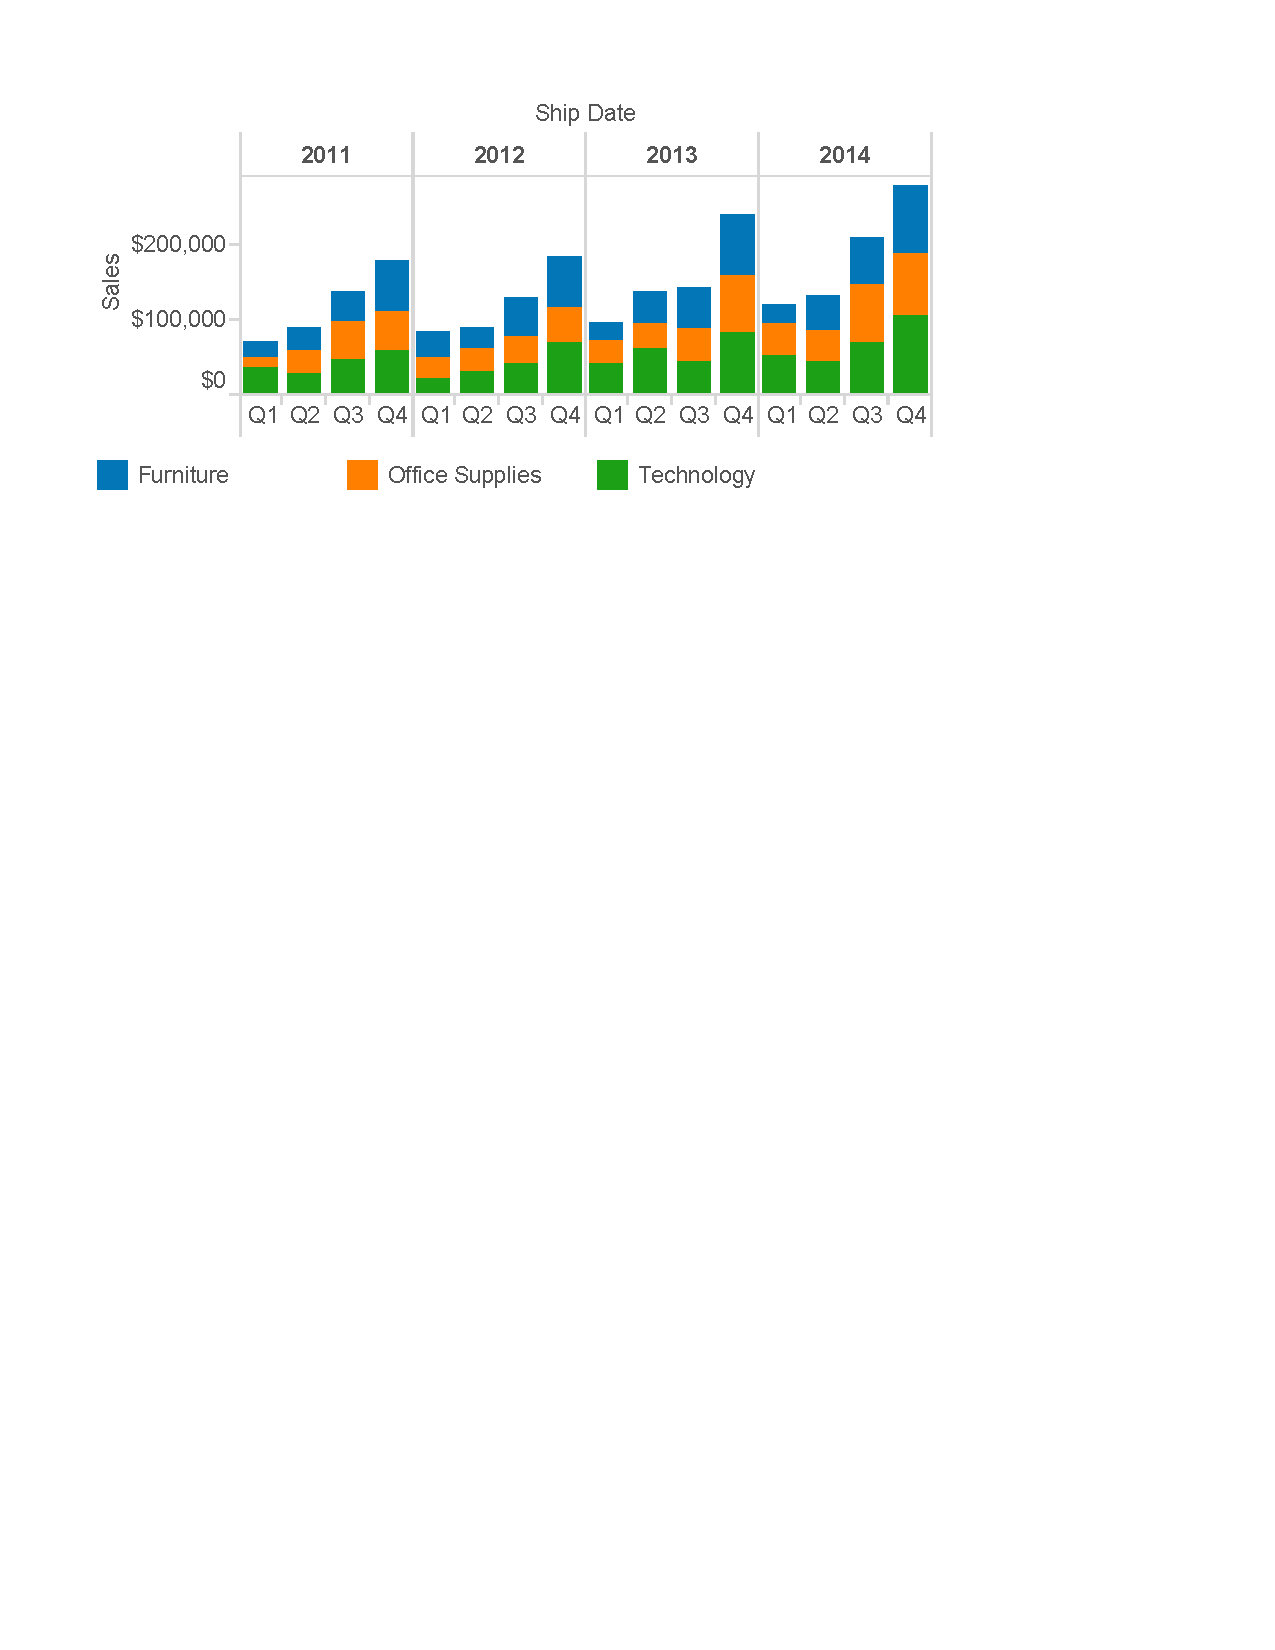
\includegraphics[width=\columnwidth]{figures/FigureI1}
\caption{Categorical Date Scalars.}
\label{fig:I1}
\end{figure}

Quantitative dates are typically used for time series on an axis that maps the underlying distance measure to display pixel distance. The quantitative analog to categorical binning is \textit{truncation} whereby all the dates in a bin are represented by the first date in the bin. Truncation accurately preserves the distance semantics while enabling roll-up to coarser levels of detail. The visualization in Figure \ref{fig:I2} shows the same sales data in a quantitative time series rolled up to the quarter level.

\begin{figure}[ht]
\centering
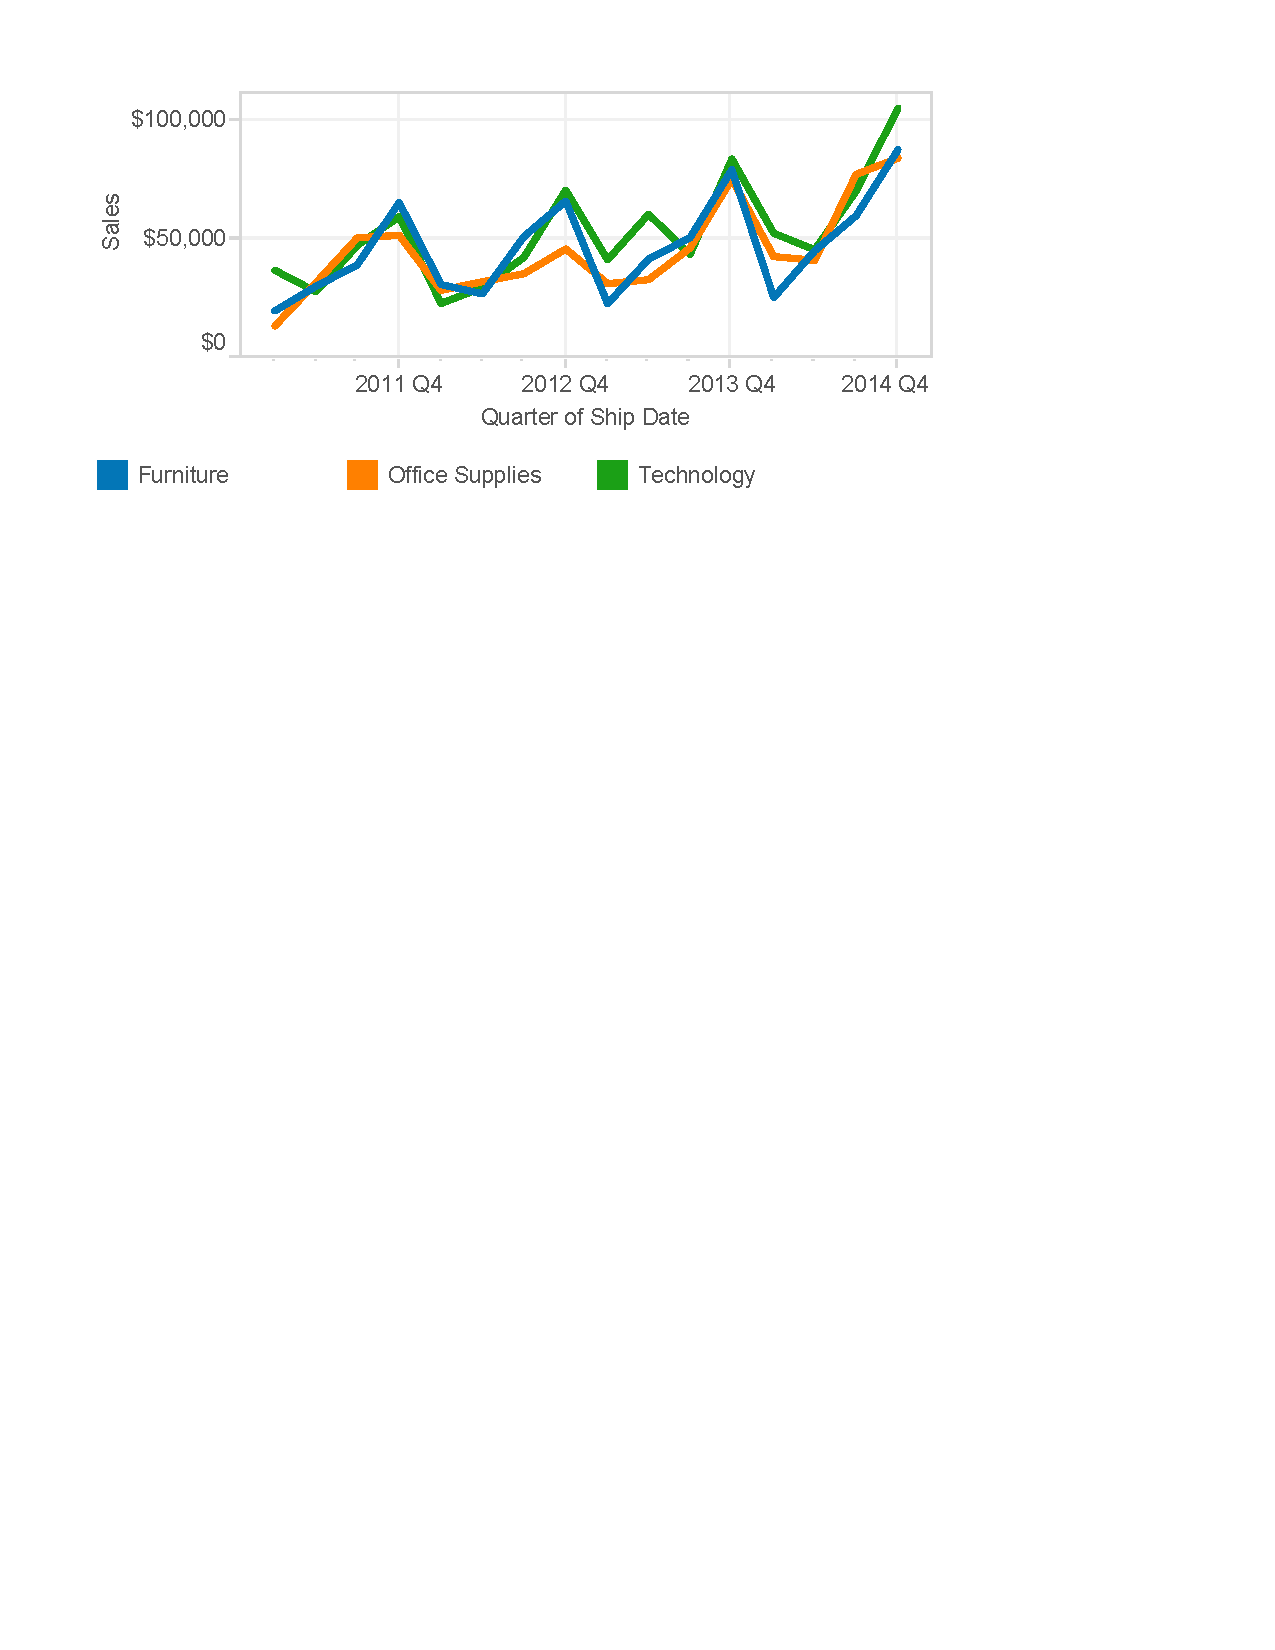
\includegraphics[width=\columnwidth]{figures/FigureI2}
\caption{Quantitative Date Scalars.}
\label{fig:I2}
\end{figure}

These types of visualizations are difficult to specify with simple categorical string representations of dates. Thus the parsing of strings to date scalars is an important form of preparation for data analytics.

\subsection{Parsing Dates}
This parsing of date representations is one of the oldest data preparation problems we have observed. A common version of this problem is how to convert columns of integers of the form \texttt{yyyyMMdd} to date scalars. Na\"{i}ve users often solve this problem by converting the integer to a string and performing some locale-dependent string operations before casting the string back to a date. Unfortunately, this approach has a number of problems:
\begin{itemize}
\setlength\itemsep{0em}
\item String operations are notoriously slow compared to scalar operations (typically 10-100x slower in modern RDBMSes)
\item Default parsing of date formats is locale-dependent, and may not work when the analysis is shared across an international organization (\eg between the US and European offices)
\item The parsing code is hard to understand and maintain because it uses a verbose, general-purpose string-handling syntax instead of a specialized domain language.
\end{itemize}

And this is but a single date format. Our studies of online data collections suggest that there are hundreds of distinct temporal date formats in user data sets. Some are common, but others can be quite idiosyncratic. Table 1 shows a selection of unusual date formats found in our corpus (the meanings of the ICU formatting codes can be found in Table 2). The first example shows a time zone in the middle of the date and a year after the time; the second shows a leading unmatched bracket and a colon between the date and time components; the third shows confusion between the seconds' decimal point and the time part delimiter; the fourth shows a two digit year apostrophe on a four digit year and the fifth shows a dash separating the date and time components. 
As can be seen in Figure \ref{fig:M2}, the long tail of formats means that these idiosyncrasies are the rule, not the exception, 
so a static enumeration of a small set of formats will not produce high reliability.

\begin{table}[ht]
\centering
\bgroup
\def\arraystretch{1.5}
\begin{tabular}{|p{0.4\linewidth}| p{0.4\linewidth}|}
\hline
\centering
\textbf{ICU Format} & \textbf{Example}\\ \hline
\scriptsize{EEE MMM dd HH:mm:ss zzz yyyy} & \scriptsize{Fri Apr 01 02:09:27 EDT 2011}\\ \hline
\scriptsize{[dd/MMM/yyyy:HH:mm:ss} & \scriptsize{[10/Aug/2014:09:30:40}\\ \hline
\scriptsize{dd-MMM-yy hh.mm.ss.SSSSSS a} & \scriptsize{01-OCT-13 01.09.00.000000 PM}\\ \hline
\scriptsize{MM ''yyyy} & \scriptsize{01 '2013}\\ \hline
\scriptsize{MM/dd/yyyy - HH:mm} & \scriptsize{04/09/2014 - 23:47}\\ \hline
\end{tabular}
\egroup
\label{tab:dateformats}
\caption{Unusual Date Formats.}
\end{table}

Several RDBMSes (\eg MySQL, Oracle and Postgres) provide row-level functions for parsing formatted dates, but our analysis of user data showed a 15\% syntax error rate using these functions. And even with perfect syntax, the user still has to interrupt her flow to learn a formatting syntax -- which she will likely forget once this specific problem has been solved.

One solution to this problem might have been to design a graphical environment that enabled users to construct valid patterns using visually compelling representations to reduce the cognitive load. This approach would have involved a substantial development effort with no guarantee that the result would be correct if the user misunderstood the environment. Moreover, this approach only solves the syntax problem -- the user is still required to switch contexts to solve their problem.

Our solution was to develop two algorithms for automatically deriving the format string from the user's data with over 95\% parsing accuracy. Both algorithms are built based on classical machine learning algorithms that learn from pattern recognition to make data-driven predictions. We developed two algorithms because we were not aware of any previous work on this problem and we needed to be able to cross-validate our results on a large testing corpus. Either approach allows the user to simply specify ``this column is a date" and the visualization system can respond quickly and accurately enough to avoid interrupting the user's cognitive flow.

\subsection{Contributions}

Specifically, our contributions include:
\begin{itemize}
\setlength\itemsep{0em}
\item By analyzing an online corpus, we provide evidence that practical date parsing requires the ability to recognize hundreds of formats;
\item We show how to extend prior work on Minimum Descriptive Length structure extraction to generate a freely available date format domain language with over 95\% accuracy;
\item We describe a second Natural Language Processing technique for generating the same date format domain language with similar accuracy. We describe how the basic algorithm is extended to support grammar variants and constraints unique to date formats. The parsing algorithm is extended to compute an overall dominant pattern over a data column;
\item We provide evidence that the development of multiple, independent parsing algorithms provides an effective means of cross-validation on large corpora;
\item We describe some limitations of this domain language that would improve its utility.
\end{itemize}

\subsection{Organization}
The rest of this paper is organized as follows: The next section provides background information for the problem space. The following two sections describe the two different algorithms, one using Minimum Descriptive Length and the other using Natural Language Processing. In section V, we evaluate the algorithms on a corpus of 30K columns, both by sampling the outputs manually and then by using the algorithms to validate each other. We then discuss related work in section VI, future work in section VII and conclude in section VIII.
